\setcounter{section}{3}
\setcounter{subsection}{2}
\setcounter{equation}{23}

\subsection{Reziproke Gitter}
	In einem periodischen Kristall sind alle relevanten Eigenschaften wie Potentiale, Elektronenkonzentrationen etc. ebenfalls periodisch.
	Es liegt daher nahe, diese Symmetrie bei der theoretischen Beschreibung zu nutzen.
\paragraph{Herleitung}
	Eine beliebige Funktion $f(\Vec{r})$ heißt periodisch, wenn gilt
	\begin{equation}
		f(\Vec{r}) = f(\Vec{r} + \Vec{t})
	\end{equation}
	mit dem Translationsvektor
	$$
	\Vec{t} = \sum_{i = 1}^{3} t_{i} \Vec{a}_{i}.
	$$
	\begin{subequations}
		Periodische Funktionen lassen sich durch eine Fourierreihe
		\begin{equation}
			\label{eq:II.3.25}
			f(\Vec{r}) = \sum_{\Vec{G} }^{} A_{\Vec{G}}\cdot e^{i \Vec{G} \Vec{r}} 
		\end{equation}
		beschreiben mit den Fourierkoeffizienten
		\begin{equation}
			A_{\Vec{G}} = \frac{1}{V_0} \int_{V_0} f(\Vec{r}) e^{-i \Vec{G} \Vec{r}},
		\end{equation}
		wobei $V_0$ dem Volumen einer primitiven Zelle im Kristall entspricht.
	\end{subequations}

	Gleichung \eqref{eq:II.3.25} ist invariant gegen eine Translation $\Vec{t}$ im realen Gitter, wenn gilt
	$$
	\sum_{\Vec{G} }^{} A_{\Vec{G}} e^{i \Vec{G} \Vec{r}} = \sum_{\Vec{G}}^{} A_{\Vec{G}} e^{i \Vec{G}\left( \Vec{r} + \Vec{t} \right) } = \sum_{\Vec{G}}^{} A_{\Vec{G}} e^{i\Vec{G} \Vec{r}} \underbrace{e^{i\Vec{G}\Vec{t}}}_{\overset{!}{=}1}~,
	$$
	also
	\begin{equation}
		\label{eq:II.3.26}
		\Vec{G} \cdot \Vec{t} = 2\pi N \qquad\text{für}\qquad N \in \mathbb{N}.
	\end{equation}

	Wir verwenden den Ansatz
	\begin{equation}
		\label{eq:II.3.27}
		\Vec{G} = h\Vec{g}_{1} + k\Vec{g}_{2} + l\Vec{g}_{3}
	\end{equation}
	mit Basisvektoren $\Vec{g}_{i}$, welche zunächst nicht näher festgelegt werden. Gleichung \eqref{eq:II.3.26} ist allgemein nur dann erfüllt, wenn
	$$
	\Vec{g}_{1} \Vec{a}_{1} = 2\pi , \quad \Vec{g}_{1} \Vec{a}_{2} = 0, \quad \Vec{g}_{1} \Vec{a}_{3} = 0 
	$$ 
	gilt, also
	\begin{equation}
		\label{eq:II.3.28}
		\Vec{g}_{i} \Vec{a}_{j} = 2 \pi \delta _{ij}.
	\end{equation}
	Die Vektoren $\Vec{G}$ geben im reziproken Gitter die erlaubten Entwicklungsglieder in der Fourierreihe vor.
	Die Fourierkoeffizienten bestimmen die Amplitude der gestreuten Strahlung.\\

	Um Gleichung \eqref{eq:II.3.28} zu erfüllen, werden die reziproken Basisvektoren definiert als
	\begin{equation}
		\label{II.3.29}
		\Vec{g}_{i} = 2\pi \frac{\Vec{a}_{j} \times \Vec{a}_{k}}{\left[ \Vec{a}_{i} \cdot\left( \Vec{a}_{j} \times \Vec{a}_{k} \right)  \right] }.
	\end{equation}
	$i,j,k$ sind zyklische Indizes und der Nenner $[\vec a_i\cdot(\vec a_j\times\vec a_k)]$ ist das Spatprodukt.\\

	$\Vec{G}$ ist ein \textbf{Translationsvektor} im \textbf{reziproken Gitter} mit den Indizes $h,k,l$. Er wird ausgedrückt als
	\begin{equation}
		\label{eq:II.3.30}
		\Vec{G}_{h,k,l} = h\Vec{g}_{1} + k\Vec{g}_{2} + l\Vec{g}_{3}
	\end{equation}
	und es gilt 
	\begin{equation}
		\label{eq:II.3.31}
		\left| \Vec{G}_{h,k,l} \right|  = \frac{2\pi}{d_{hkl}} .
	\end{equation} 

	\begin{verbal}
		Die genaue Herleitung ist in Hunklingers \textit{Festkörperphysik} ab Seite 99 zu finden.
	\end{verbal}
	Das reziproke Gitter wird also aufgebaut aus drei Basisvektoren in Richtung der Senkrechten zu den drei Ebenen, die durch jeweils ein Paar der Basisvektoren des realen Gitters gebildet werden.

\paragraph{Streuung im reziproken Gitter}

	Setzt man den Vektor $\Delta \Vec{k}$, der in der Laue Gleichung \eqref{eq:II.3.19} auftaucht, gleich einem beliebigen Vektor des reziproken Gitters, so werden die Bedingungen für die Interferenzmaxima und Beachtung von Gleichung \eqref{eq:II.3.28} automatisch erfüllt.
	Dort gilt die
	\begin{important}
		Bedingung für ein Interferenzmaximum\\
		\begin{equation}
			\label{eq:II.3.32}
			\Delta k = \Vec{G}.
		\end{equation}
	\end{important}

	Der Streuvektor ist gleich einem reziproken Gittervektor. Sie Streubedingung lässt sich somit durch die sogenannte {Ewald-Kugel} im reziproken Raum veranschaulichen. Sie ist in \autoref{fig:vl17_ewald_kugel} dargestellt und erklärt.\\

	\begin{figure}[H]
		\centering
		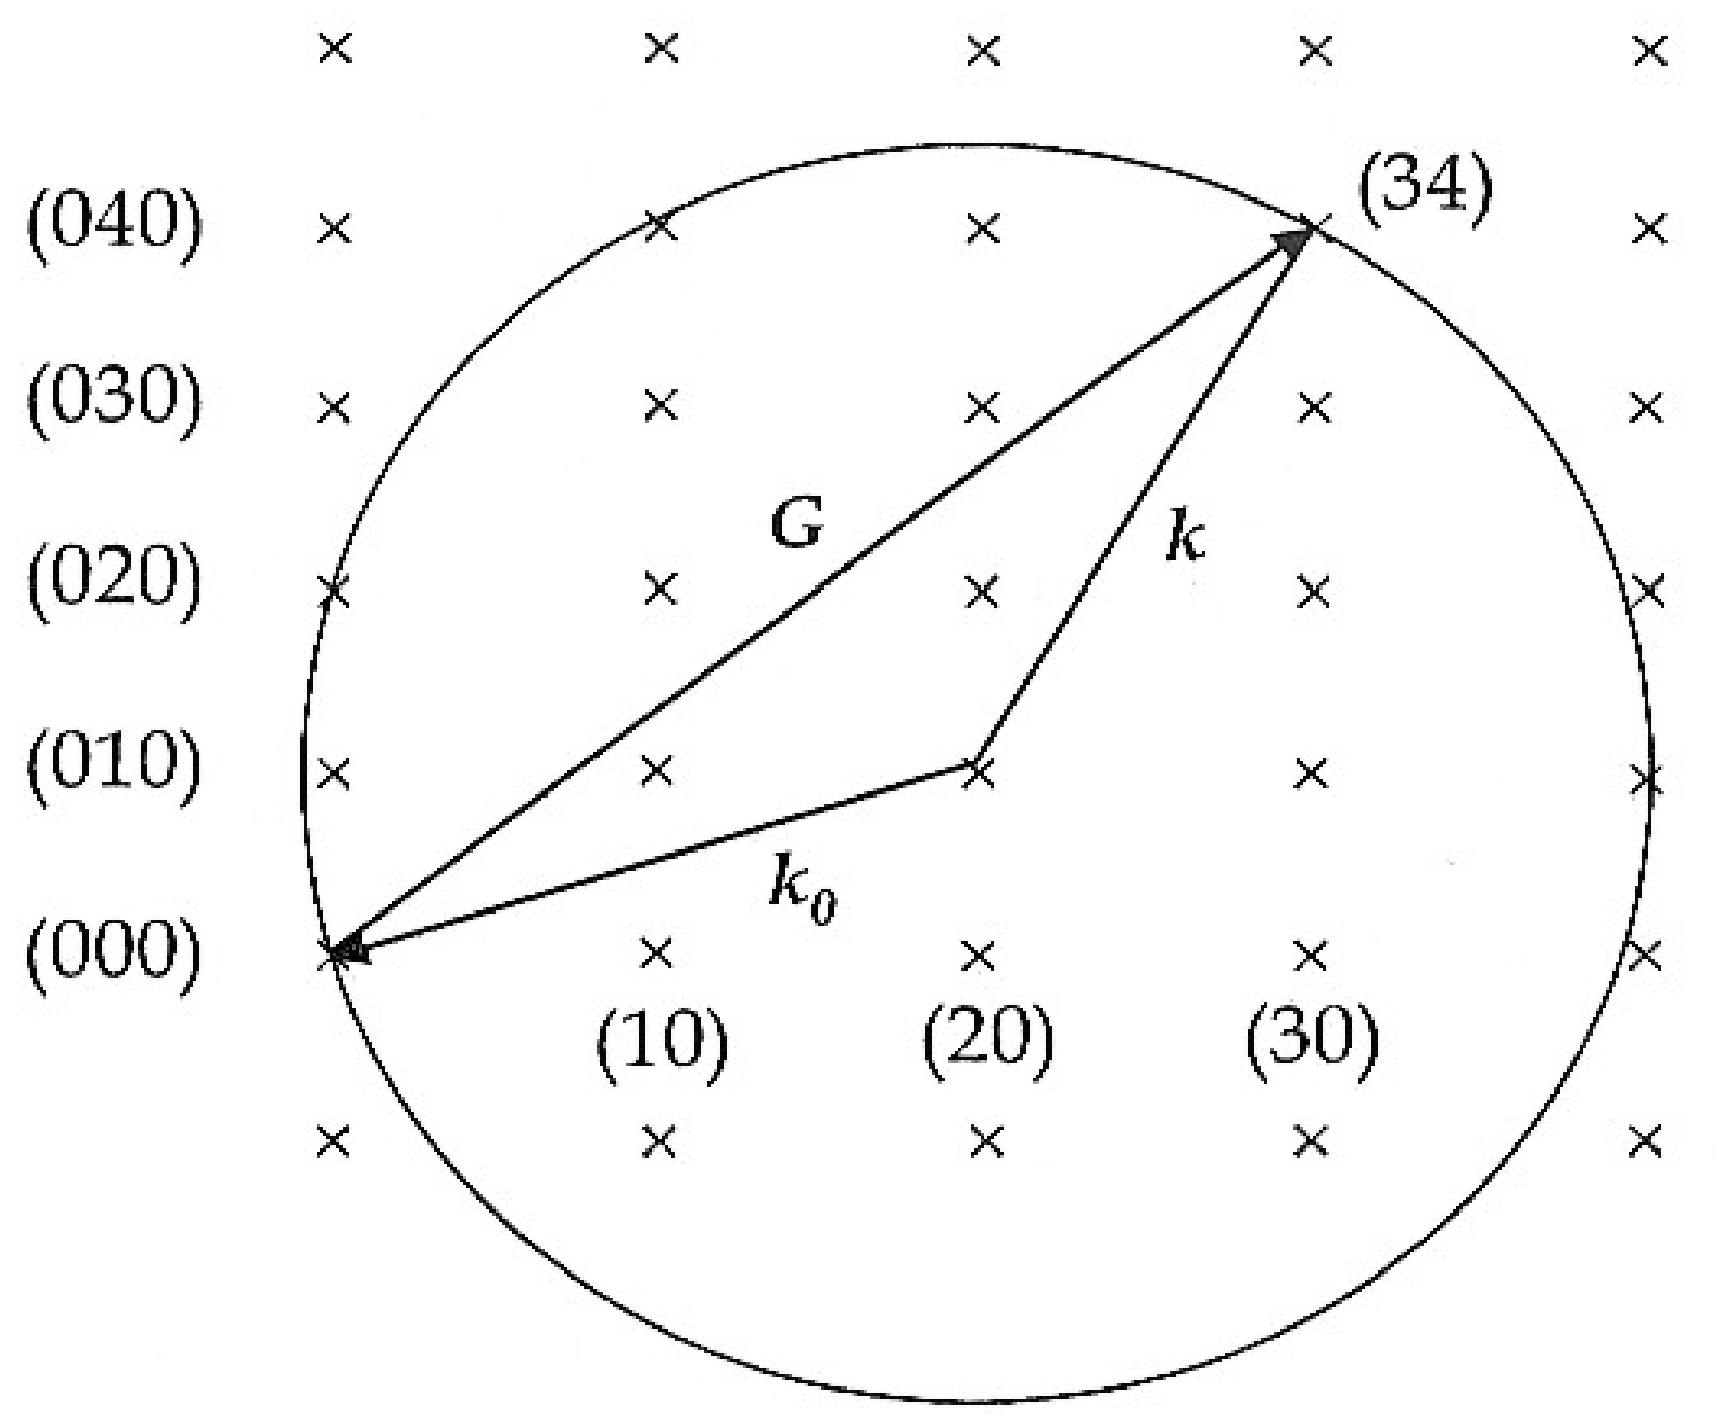
\includegraphics[width=0.5\linewidth]{figures/vl17/ewald-kugel.png}
		\caption{Ewald-Kugel und Beugung eines einfallenden Strahles im reziproken Gitter. \cite{Ibach}.\\
			Die Kreuze sind reziproke Gitterkoordinaten $(xyz)$, bzw $(xy)$. 
			$\vec k_0$ ist die Wellenzahl des einfallenden Lichtstrahls.
			Am Ende von $\vec k_0$ liegt das Zentrum der Kugel mit Radius $|k_0|$.
			Diese Kugel heißt Ewald-Kugel.\\
			Vom Zentrum geht ein zweiter Vektor $\vec k$ zu einem Gitterpunkt auf der Kugeloberfläche (in diesem Falle zu $(34)$).
			$\vec k$ ist der Wellenvektor des ausfallenden (gebeugten) Strahls, da die Wellenvektoren der Beugungsbedingung \eqref{eq:II.3.32} genügen.
		}
		\label{fig:vl17_ewald_kugel}
	\end{figure}
\paragraph{Gitteranalyse}
	Bei der Beugung erhält man ein Abbild des reziproken Gitters. Es können Intensitäten gemessen werden, jedoch gehen Phaseninformation verloren.
	Die Verteilung der Streudichte kann deshalb nicht unmittelbar berechnet werden. Im praktischen Vorgehen werden ausgehend von einem Strukturvorschlag die Beugungsintensitäten berechnet, welche dann mit den experimentellen Daten verglichen werden. Bei Abweichungen werden Anpassungen vorgenommen und der Prozess wird wiederholt, bis es zu einer Übereinstimmung kommt.

\paragraph{Brillouin-Zone}
	Im reziproken Gitter kann man auch eine Elementarzelle konstruieren. Die Wigner-Seitz-Zelle der reziproken Gitters wird Brillouin-Zone genannt.\\

	Um diese zu erhalten, schreiben wir die Beugungsbedingung \eqref{eq:II.3.32} um:
	$$
	\begin{aligned}
		&& \Delta \Vec{k} &= \Vec{G} \\
		&\Leftrightarrow& \Vec{k} + \Vec{G} &= \Vec{k}' \\
		&\Leftrightarrow& \left( \Vec{k} + \Vec{G} \right) ^2 &= k'^2 \qquad\text{mit} \left| \Vec{k}' \right| = \left| \Vec{k} \right|: \\
		&\Leftrightarrow& 2 \Vec{k} \Vec{G} + \Vec{G}^2 &= 0
	\end{aligned}
	$$
	Wenn $\Vec{G}$ ein reziproker Gittervektor ist, dann gilt dies auch fúr $-\Vec{G}$:
	\begin{align}
		2 \Vec{k} \Vec{G} &= G^2 \nonumber\\
		\Vec{k} \left( \frac{1}{2} \Vec{G} \right)  &= \left( \frac{1}{2} G \right) ^2 \nonumber
	\end{align}
	Durch Umformen erhalten wir die
	\begin{important}
		Darstellung der Beugungsbedingung durch {Brillouin}\\
		\begin{equation}
			\Vec{k} \Vec{G} = \frac{1}{2} G^2 \label{eq:II.3.33}.
		\end{equation}
	\end{important}
	\autoref{fig:vl17_brillouin_2d} zeigt die Brillouin-Zonen in einem 2-dimensionalen Gitter, \autoref{fig:vl17_brillouin_3d} in einem 3-dimensionalen Gitter.
	\begin{figure}[H]
		\centering
		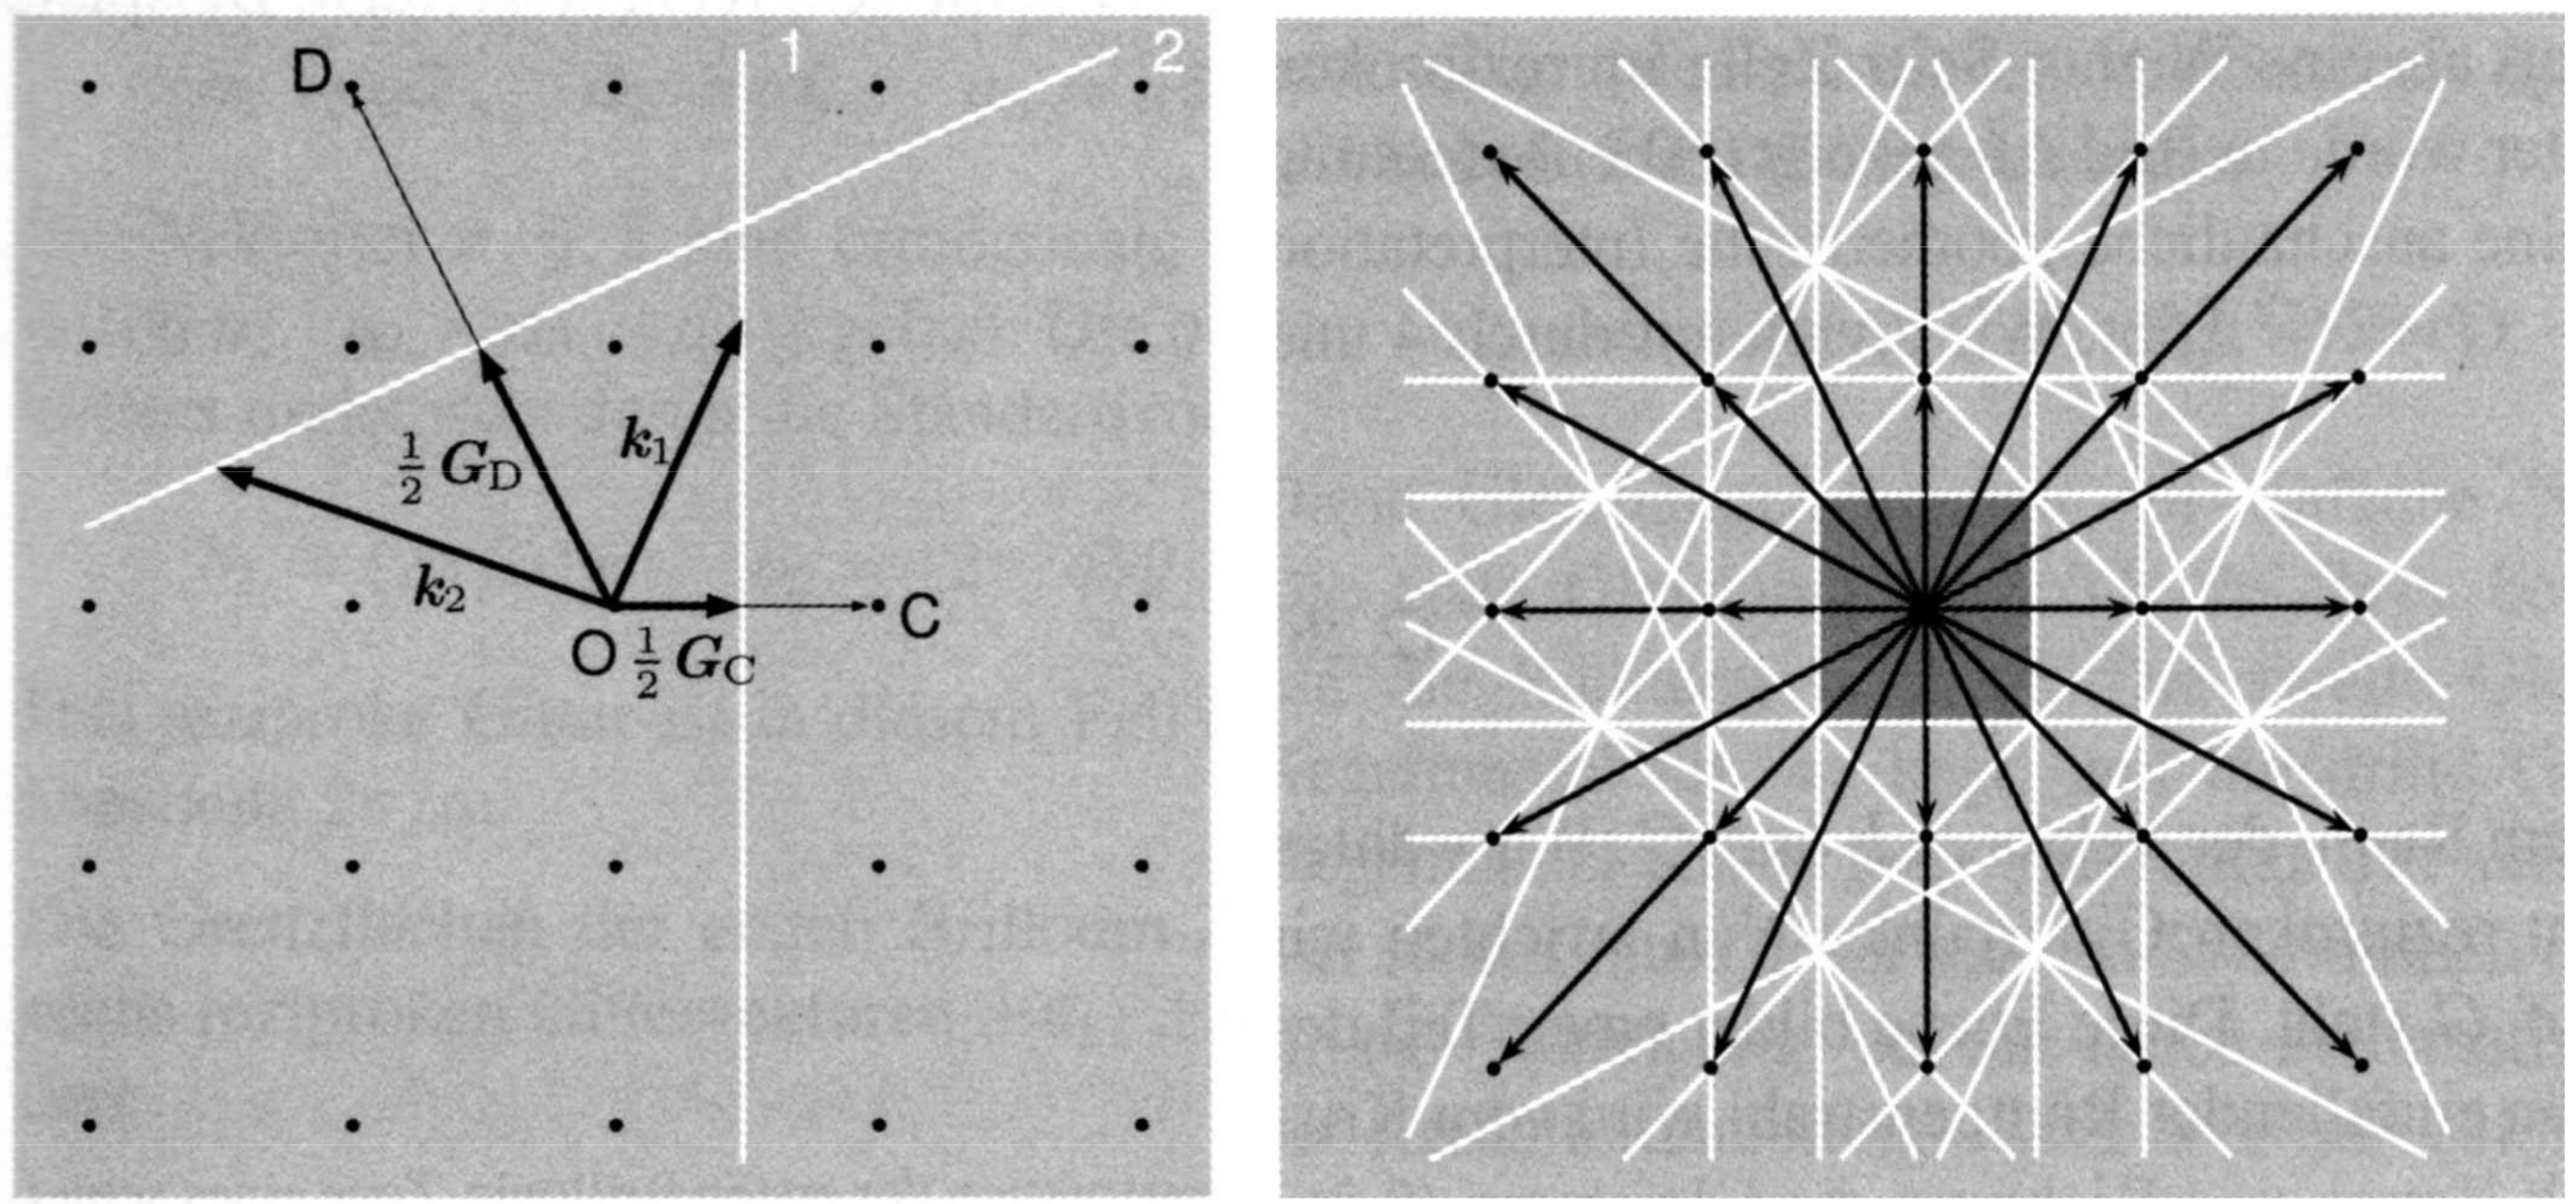
\includegraphics[width=0.8\linewidth]{figures/vl17/brillouin_zonen_2d.png}
		\caption{Brillouin-Zonen eines 2-dimensionalen Giters \cite{Kittel}. 
			Die Gittervektoren $\vec G_{C,D}$ verbinden die Punkte $0$ und $C$, bzw $D$. 
			Auf halber Länge der Gittervektoren wird senkrecht eine Brillouin-Zone aufgespannt.
			Alle Wellenvektoren $\vec k_i$, welche auf einer Brillouin-Zone liegen, genügen der Beugungsbedingung \eqref{eq:II.3.33}.
		}
		\label{fig:vl17_brillouin_2d}
	\end{figure}
	\begin{figure}[H]
		\centering
		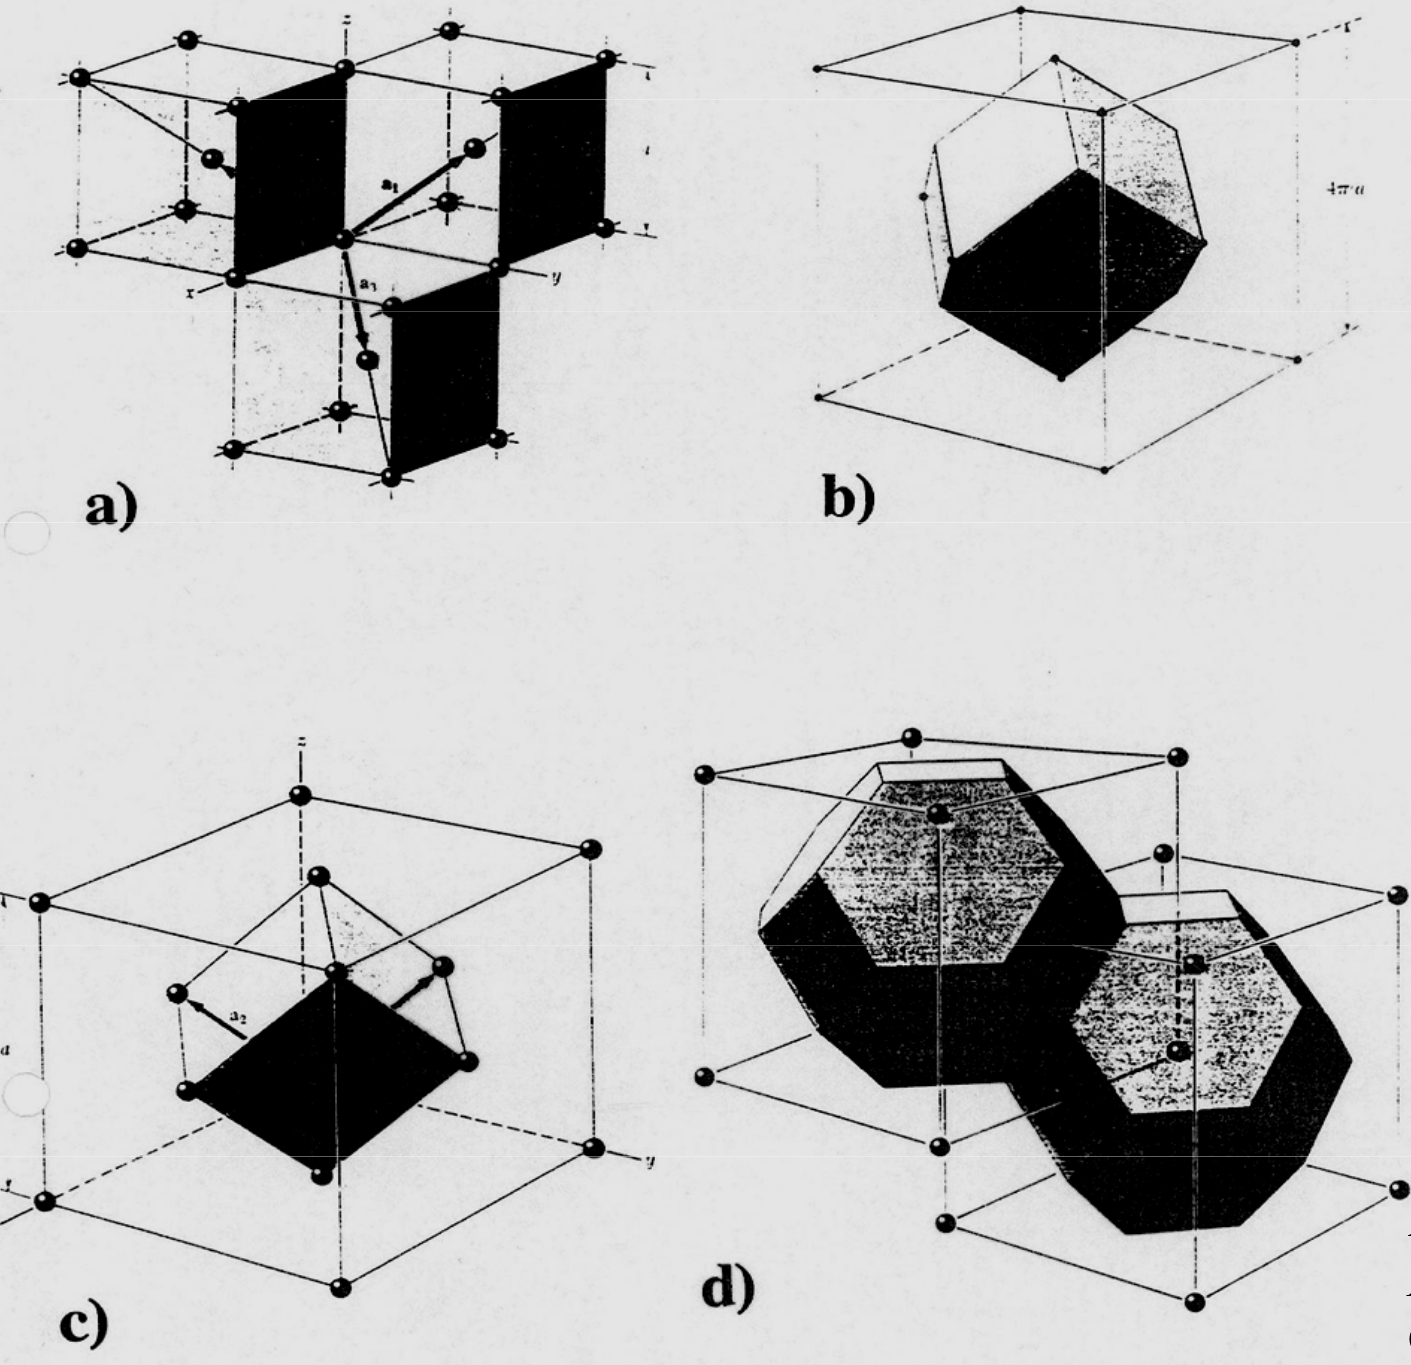
\includegraphics[width = 0.6\linewidth]{figures/vl17/brillouin_zonen_3d.png}
		\caption{Brillouin-Zonen eines 3-dimensionalen Gitters \cite{Kittel}.}
		\label{fig:vl17_brillouin_3d}
	\end{figure}

\paragraph{Geometrische Interpretation}
	Sei $\varphi$ der Winkel zwischen dem Wellenvektor $\vec k$ und dem halbierten Gittervektor $\vec G/2$.
	Falls $\Vec{k}$ auf den Rand der Brillouin-Zelle fällt, ist 
	$$\cos\varphi =\frac{G/2}{k}$$ 
	und somit
	$$\vec k\cdot\vec G= kG\cos\varphi = kG\frac{G/2}{k}=\frac{1}{2}G^2.$$
	Damit weißt die Brillouinkonstruktion alle Wellenvektoren $\Vec{k}$ auf, die vom Kristall {reflektiert} werden können.

\paragraph{Bemerkung}
	Das reziproke Gitter ist wichtig im Bereich der Wellenausbreitung, Behandlung von Richtungen, Impulsen etc., z.B. Elektronen im Kristall.

\paragraph{Intensitäten der reflektierten Strahlen}
	Die Streubedingungen \eqref{eq:II.3.32} und \eqref{eq:II.3.33} besagen zunächst nur, wo Reflexe auftreten. 
	Um Aussage über die Intensitäten zu machen muss man die lokale Elektronendichteverteilung berücksichtigen.

	Dazu nehmen wir an, dass an den Gitterpunkten der Elementarzelle unterschiedliche Atome liegen können. Die Basis ist also mehratomig.

	Die Standorte der Atome sind gegeben durch
	\begin{equation}
		\label{eq:II.3.34}
		\Vec{R} = \Vec{R}_{m,n,p} + \Vec{\rho}_{j} = \left( m + u_{j} \right) \Vec{a} + \left( n + v_{j} \right) \Vec{b} + \left( p + w_{j} \right) \Vec{c}
	\end{equation}
	mit $m,n,p$ ganzzahlig und $u_{j}, v_{j}, w_{j} $ nicht ganzzahlig. 
	$\vec R_{m,n,p}$ ist somit ein primitiver Gittervektor und $\vec\rho_j$ die Verbindung zu Atomen, welche nicht mit mit $\vec R_{m,n,p}$ erreichbar sind.

	Einsetzen in Gleichung \eqref{eq:II.3.18} liefert
	\begin{equation}
		\Vec{E} (\Vec{r}) = \Vec{A}\,' (\Vec{r}) \sum_{m,n,p = 0}^{Z-1} \sum_{j = 1}^{S} f_{j} \exp\left( i \Delta \Vec{k} \left[ \left( m + u_{j} \right) \Vec{a} + \left( n + v_{j} \right) \Vec{b} + \left( p + w_{j} \right) \Vec{c}\,\right]  \right) e^{i\Vec{k} \Vec{r}}.
		\label{eq:II.3.35}
	\end{equation}
	Der Atomformfaktor $f_j$ berücksichtigt das spezifische Streuvermögen der Elektronenhüllen chemisch unterschiedlicher Atome. 
	Wird der Festkörper mit Neutronen beschossen, berücksichtigt er die Wechselwirkungen der Neutronen mit den Kernen.

	Aus Gleichung \eqref{eq:II.3.35} folgt
	\begin{equation}
		\label{eq:II.3.36}
		\begin{split}
			\Vec{E} (\Vec{r}) = \Vec{A}\,'(\Vec{r}) \Bigg[ \sum_{j = 1}^{S}  f_{j} e^{i \Delta \Vec{k} \left( u_{j} \Vec{a} + v_{j} \Vec{b} + w_{j} \Vec{c} \right) }  \Bigg] 
			\cdot \Bigg[ \sum_{m,n,p}^{} e^{i \Delta \Vec{k} \left( m \Vec{a} + n \Vec{b} + p \Vec{c} \right) }   \Bigg] e^{i\Vec{k}\Vec{r}}.
		\end{split}
	\end{equation}
	Für das Auftreten von Reflexen gilt
	$$
	\Delta \Vec{k} = \Vec{G}_{hkl} = h \Vec{g}_{1} + k\Vec{g}_{2} + l\Vec{g}_{3}.
	$$ 
	Setzen wir diese Bedingungen in Gleichung \eqref{eq:II.3.36} ein, erhalten wir den Strukturfaktor
	\begin{equation}
		\label{eq:II.3.37}
		F = \sum_{j = 1}^{S}  f_{j} e^{2\pi i \left( hn_{j} + kv_{j} + lw_{j} \right) }.
	\end{equation}
\paragraph{Strukturfaktor}
	Der Strukturfaktor $F$ beschreibt innere Interferenzen einer mehratomigen Basis (Einheitszelle).

	{Beispiel:} Betrachte ein kubisch raumzentriertes Gitter mit zwei Atomen je Elementarzelle mit Koordinaten $\left( 0,0,0 \right) $ und $\left( \frac{1}{2}, \frac{1}{2}, \frac{1}{2} \right) $.
	\begin{enumerate}
		\item Sind die Atome identisch, dann ist $f_1 = f_2$. Der Strukturfaktor lautet demnach
			$$
			F\left( h,k,l \right) = f_1 \left( 1 + e^{i \pi \left( h+k+l \right) } \right) 
			$$ 
			und damit
			$$
			F = \begin{cases}
				0 & \text{für } h+k+l \text{ ungerade}\\
				2f_1 & \text{für } h+ k+l \text{ gerade}
			\end{cases}
			$$ 
			Im Beugungsdiagramm verschwinden alle Reflexe mit ungerader Indexsumme.
		\item Sind die Atome verschieden, so ist der Strukturfaktor
			$$F\left( h,k,l \right) = f_1 +f_2 e^{i \pi \left( h+k+l \right) }$$
			und
			$$
				F = \begin{cases}
					f_1 - f_2 \qquad h+k+l \text{ ungerade}  	&\quad \to \text{schwacher Reflex} \\
					f_1 + f_2 \qquad h+k+l \text{ gerade} 		&\quad \to \text{starker Reflex}
				\end{cases}
			$$ 
	\end{enumerate}
	Für die Reflektion ist also nicht nur die räumliche Anordnung der Atome wichtig, sondern auch deren Art. 
	\autoref{fig:vl17_diffraktogramm} zeigt, wie sich das Reflektionsverhalten von Festkörpern mit gleicher Gitterform aber unterschiedlichen Phasen (geordnet bzw. ungeordnet) unterscheiden kann.

	\begin{figure}[H]
		\centering
		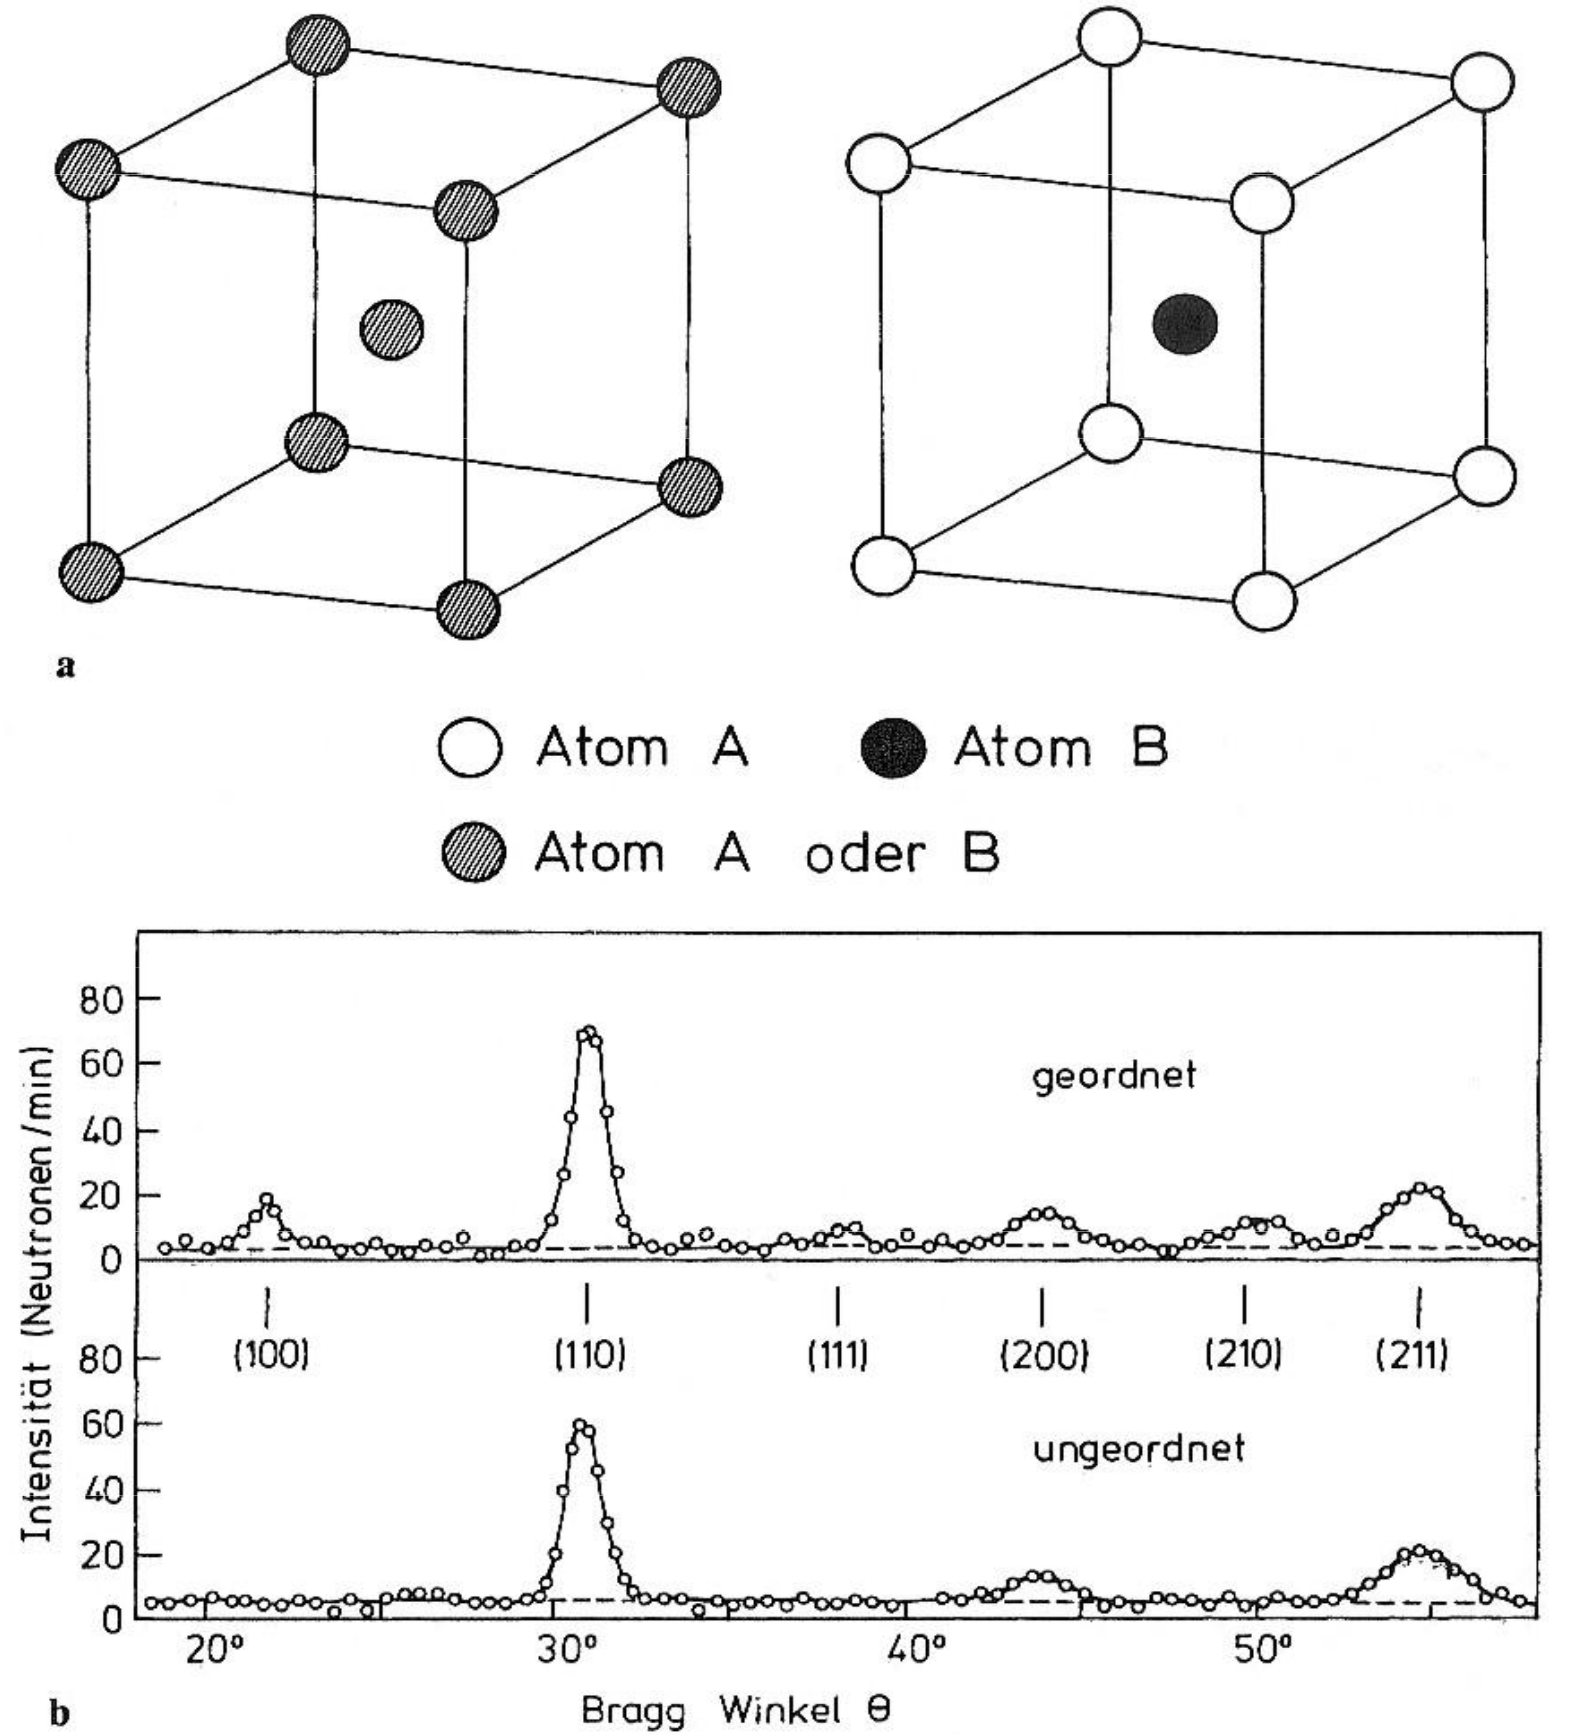
\includegraphics[width = 0.7 \linewidth]{figures/vl17/diffraktogramm.png}\
		\caption{Neutronen-Diffraktogramm einer geordneten und ungeordneten Phase von \ce{FeCo} \cite{Ibach}.
			Das linke Gitter ist ungeordnet und entsteht bei schneller Abkühlung.
			Das rechte Gitter ist geordnet und entsteht, wenn der Körper bei langsamer Abkühlung kristallisiert.
			Die Diffraktogramme der beiden Phasen unterscheiden sich.
		}
		\label{fig:vl17_diffraktogramm}
	\end{figure}
	Im ungeordneten Fall entfallen die Reflexe mit ungerader Indexsumme (siehe obige Diskussion).